\documentclass[11pt]{iopart}
%Uncomment next line if AMS fonts required
%\usepackage{iopams}
\usepackage{fancyhdr}
\usepackage{graphicx}
\usepackage{todonotes}
\usepackage{subfig}
\usepackage{ulem}
\usepackage{amssymb}
\usepackage{multicol}

\usepackage[hidelinks]{hyperref}
\hypersetup{colorlinks=false}

\usepackage[font={small}]{caption}

\pagestyle{fancy}
\lhead{Diffusion Limited Aggregation}
\rhead{Candidate Number: 21594}

\begin{document}

%Makes TODO notes format properly in margin
\setlength{\marginparwidth}{1.5cm}

\title[]{The Ising Model}

\author{Candidate Number: 21594}

\address{Department of Physics,
University of Bath, Bath BA2 7AY, United Kingdom}
\begin{abstract}
TODO
\end{abstract}

%\listoftodos

%Uncomment for PACS numbers title message
%\pacs{00.00, 20.00, 42.10}
% Keywords required only for MST, PB, PMB, PM, JOA, JOB? 
%\vspace{2pc}
%\noindent{\it Keywords}: Article preparation, IOP journals
% Uncomment for Submitted to journal title message
%\submitto{\JPA}
% Comment out if separate title page not required
%\maketitle

\section*{Preface}
Although the coursework was initially presented as a C++ project, I took the liberty of rewriting the Ising Model system in a programming language called Google Go (https://golang.org). The motivation for this is Go has been designed to accommodate systems with high concurrency. This means that instead of simulating 1 system at a time, 10,000 different systems can be simulated simultaneously in different threads. This greatly increases time efficiency and has allowed me to achieve a significant level of statistical significance in my ensemble averages. Furthermore, this has also allowed me to use ergodicity to calculate time averages for the same system with many different values of beta at the same time. To achieve the highest possible concurrent number of simulations, the results presented here were generated on a 32-core virtual private server. The source code for my implementation is accessible on Github: \url{http://tiny.cc/brb75y}.

\section{Introduction and Computational Method}
Ferromagnetism is the property of a material to exhibit speontaneous magnetisation in the absence of an external magnetic field. The Ising Model is a mathematical model that uses the results of thermodynamics and statistical mechanics to describe how magnetic structure in some metals leads to ferromagnetism.

In the Ising Model presented in this paper, a magnetic material is modelled by a regular $L$ x $L$ dimensional square lattice $\Pi$. A given grid point on this lattice $\pi_{(i,j)} \in \Pi$ is indexed by cartesian coordinates $(i, j)$ where $i, j \in [0, L]$. These coordinates are not strictly unique as periodic boundary conditions are applied so that a closed system is modelled. This is to say the grid follows the mappings $(i + \Lambda_i D, j + \Lambda_j D) \to (i, j)$ for $\Lambda_i, \Lambda_j \in \mathbb{Z}$. Each grid point $\pi_{(i, j)} \in \Pi$ on this square lattice is assigned a discrete variable  $s_{(i, j)} \in \{0, 1\}$ that corresponds to the spin of the grid point. The system is therefore composed of $N \equiv L^2$ spins. We arbitrarily define $s_{(i, j)} = 1$ to represent 'spin up' and $s_{(i,j)} = -1$ to represent 'spin down'.

\begin{figure}[b]
  \centering
  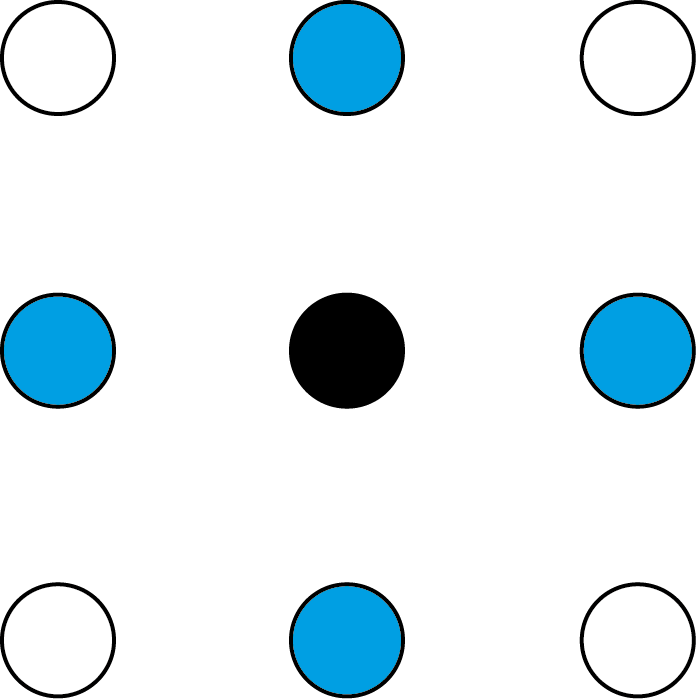
\includegraphics[width=0.10\linewidth]{images/nearestneighbour/4x/nearestneighbour@4x.png}
  \caption{Each dot represents a grid point on the square lattice $\Pi$. The central black grid point represents the grid point $\pi_{(i, j)}$. The blue grid points represent the nearest neighbours of $\pi_{(i, j)}$. The white grid points represent points that are not considered nearest neighbours.}
  \label{fig:nearestneighbours}
\end{figure}

For a given grid point $\pi_{(i, j)}$, the convention of nearest neighbours is defined as representing the grid points directly adjacent to the grid point, both vertically and horizontally, as shown in Figure \ref{fig:nearestneighbours}. Using this convention, the energy of a given spin on the grid is defined by
\begin{equation}
E_{(i, j)} = -h_{(i, j)} s_{(i, j)}
\end{equation}
where
\begin{equation}
h_{(i, j)} = \sum_{(\alpha, \beta) \; \textrm{\small{n.n. of}} \; (i, j)} \left[ J  s_{(\alpha, \beta)} \right]
\end{equation}
Here "n.n" represents a sum over the nearest neighbours and $J$ is a positive real number with dimensions of energy that indicates the strength of the interactions between spins. Qualitatively this set of equations defines the energy of a given spin as the sum of the interaction energies between the spin and it's nearest neighbours, where the interaction energy between two nearest neighbour spins is defined to be $-J$ if the two spins are aligned and $+J$ if the two spins are antiparallel, as shown in Figure \ref{fig:spinalignment}.

From this definition of the energy for a single spin in the system, the total energy for the system is defined as
\begin{equation}
\label{eq:systemenergy}
E = \frac{1}{2} \sum_{i, j} E_{(i, j)}
\end{equation}
where the summation simply runs over every grid point in the square lattice.
Furthermore, the magnetisation (per spin) of the system is defined as
\begin{equation}
\mathcal{M} = \frac{1}{N} \sum_{i, j} s_{(i, j)}
\end{equation}

\begin{figure}[t]
  \centering
  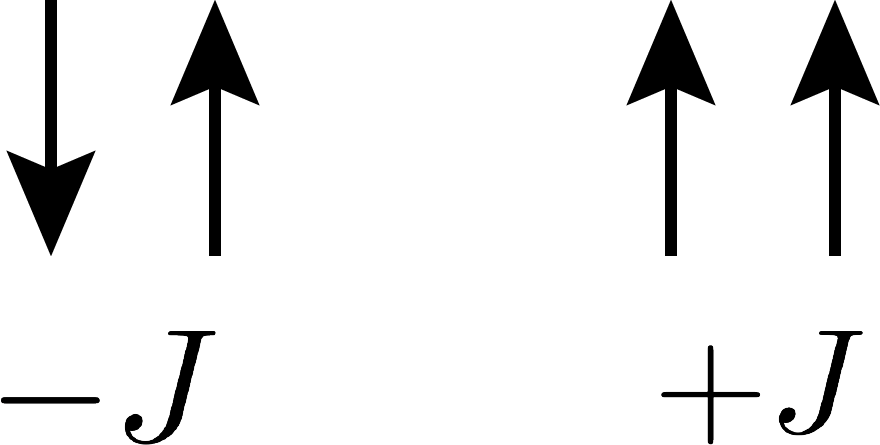
\includegraphics[width=0.2\linewidth]{images/spins/4x/spins@4x.png}
  \caption{Two nearest neighbour spins on the grid have an interaction energy of $-J$ if they are aligned and $+J$ if they are not aligned.}
  \label{fig:spinalignment}
\end{figure}

As the number of spins in the system is fixed, a canonical thermodynamic ensemble is used. If we let a microstate $\mathcal{S}$ be defined by the instantaneous configuration of all the spins in the system, then the probability of finding the system in a microstate $S$ in thermal equilibrium at temperature $T$ is given by statistical mechanics as
\begin{equation}
p_{eq}(\mathcal{S}) = \frac{1}{Z(T)} e^{-E(S)/k_B T}
\end{equation}
where $E(S)$ is the energy of microstate $S$ as given by equation (\ref{eq:systemenergy}). The canonical partition function $Z = Z(T)$ is used to enforce the normalisation condition $\sum_S{p_{eq}(S)} = 1$ which gives the expression for $Z$ as
\begin{equation}
Z(T) = \sum_{S} e^{-E(S)/k_B T}
\end{equation}
where the summations here run over all $2^N$ possible microstates $S$ of the system.

In this paper, a Metropolis Monte Carlo method is used to investigate the properties $E$ and $\mathcal{M}$ of two dimensional Ising Model systems for different thermodynamic temperatures $T$.  

\section{Method}

\subsection{Calculating Equilibrium Averages}

Instead of calculating averages using an ensemble average as is conventional for statistical mechanical systems, it is in most cases also possible to calculate an average $\langle \Gamma \rangle$ for a quantity of interest $\Gamma$ by taking a time average, where time is proportional to the number of Monte Carlo sweeps completed in our case. This is the principle of the ergodic hypothesis of thermodynamics \cite{statmech}.  For the case of a simulated Ising system, this means that average values can be determined by running a single simulation for a period of time as opposed to running many distinct simulations of that one system. In this way, an average value $\langle \Gamma \rangle$ is determined by taking $n$ samples $\{ \Gamma_i \}_{i=1}^{n}$ over a period of time. The average value is then calculated by
\begin{equation}
\label{eq:averages}
\langle \Gamma \rangle = \frac{1}{n}\sum_{i=1}^{n} \Gamma_i
\end{equation}
For independent measurements, then the uncertainty in this average is estimated well by the standard error
\begin{equation}
\label{eq:standarderror}
\bar{\sigma}_{\Gamma} = \frac{1}{\sqrt{n-1}} \sqrt{ \frac{1}{n} \sum_{i=1}^{n} \left( \Gamma_i - \langle \Gamma \rangle \right)^2 }
\end{equation}

When calculating equilibrium averages for properties of an Ising system, it is important to ensure the system has reached thermodynamic equilibrium before starting to take samples of the quantity being averaged. For all equilibrium averages presented in this paper, an integer $n_0$ of Monte Carlo cycles are waited before samples are contributed to an average. This is to give the system time to evolve through its initial transient behaviour as the system changes from the initial all spin down configuration to a state of equilibrium characterised by the thermodynamic temperature of the system.

As the Metropolis Monte Carlo simulation used in this paper is based on a Markovian random walk of phase space, subsequent samples of $\Gamma$ are very likely to exhibit autocorrelation. Consequently, if a time average $\langle \Gamma \rangle$ is to be representative of the system's entire equilibrium distribution for a practical number of samples $n$, it is useful to only sample $\Gamma$ every $\Delta \in \mathbb{Z}^{+}$ Monte Carlo sweeps. This increases the likelihood that subsequent samples are independent.

So, to account for both initial transient behaviour and to reduce the effect of autocorrelation, samples for equilibrium averages in this paper are taken at Monte Carlo times (sweep numbers)
\begin{equation}
t_i = n_0 + i \Delta
\end{equation}  

\subsection{Calculating Derived Quantities}

It can be shown that the specific heat capacity $c$ and the magnetic susceptibility $\chi$ of an Ising system are determinable by the equations \cite{handout}
\begin{equation}
c = \frac{1}{N k_B T^2} \textrm{Var}(E)
\end{equation}
\begin{equation}
\chi = \frac{N}{k_B T} \textrm{Var}({\mathcal{M}})
\end{equation}
where $k_B$ is the Boltzmann constant, $T$ is the thermodynamic temperature of the Ising system and $\textrm{Var}(E)$ and $\textrm{Var}(\mathcal{M})$ refer to the variance of the system energy and magnetisation respectively.

\section{Results}

\subsection{Convergence to Equilibrium}

An Ising model simulation was prepared with all spins initially down. For different values of system temperature, as defined by the parameter $\beta$, the system was computationally simulated using the Metropolis Monte Carlo algorithm. The system's magnetisation per spin $\mathcal{M}$ and dimensionless energy $E/J$ were recorded as the number of Monte Carlo sweeps of the system was increased from 0 to 50. For each value of $\beta$, this simulation was run for an ensemble of $10,000$ independent sub-systems, each with different pseudo-random number generator seeds. The evolution of system magnetisation as the number of Monte Carlo sweeps completed increases is shown in Figure \ref{fig:magnetisationconvergence}. Similarly, Figure \ref{fig:energyconvergence} shows the evolution of the system's dimensionless energy $E/J$ as the number of Monte Carlo sweeps increases.

\begin{figure}[t]
  \centering
  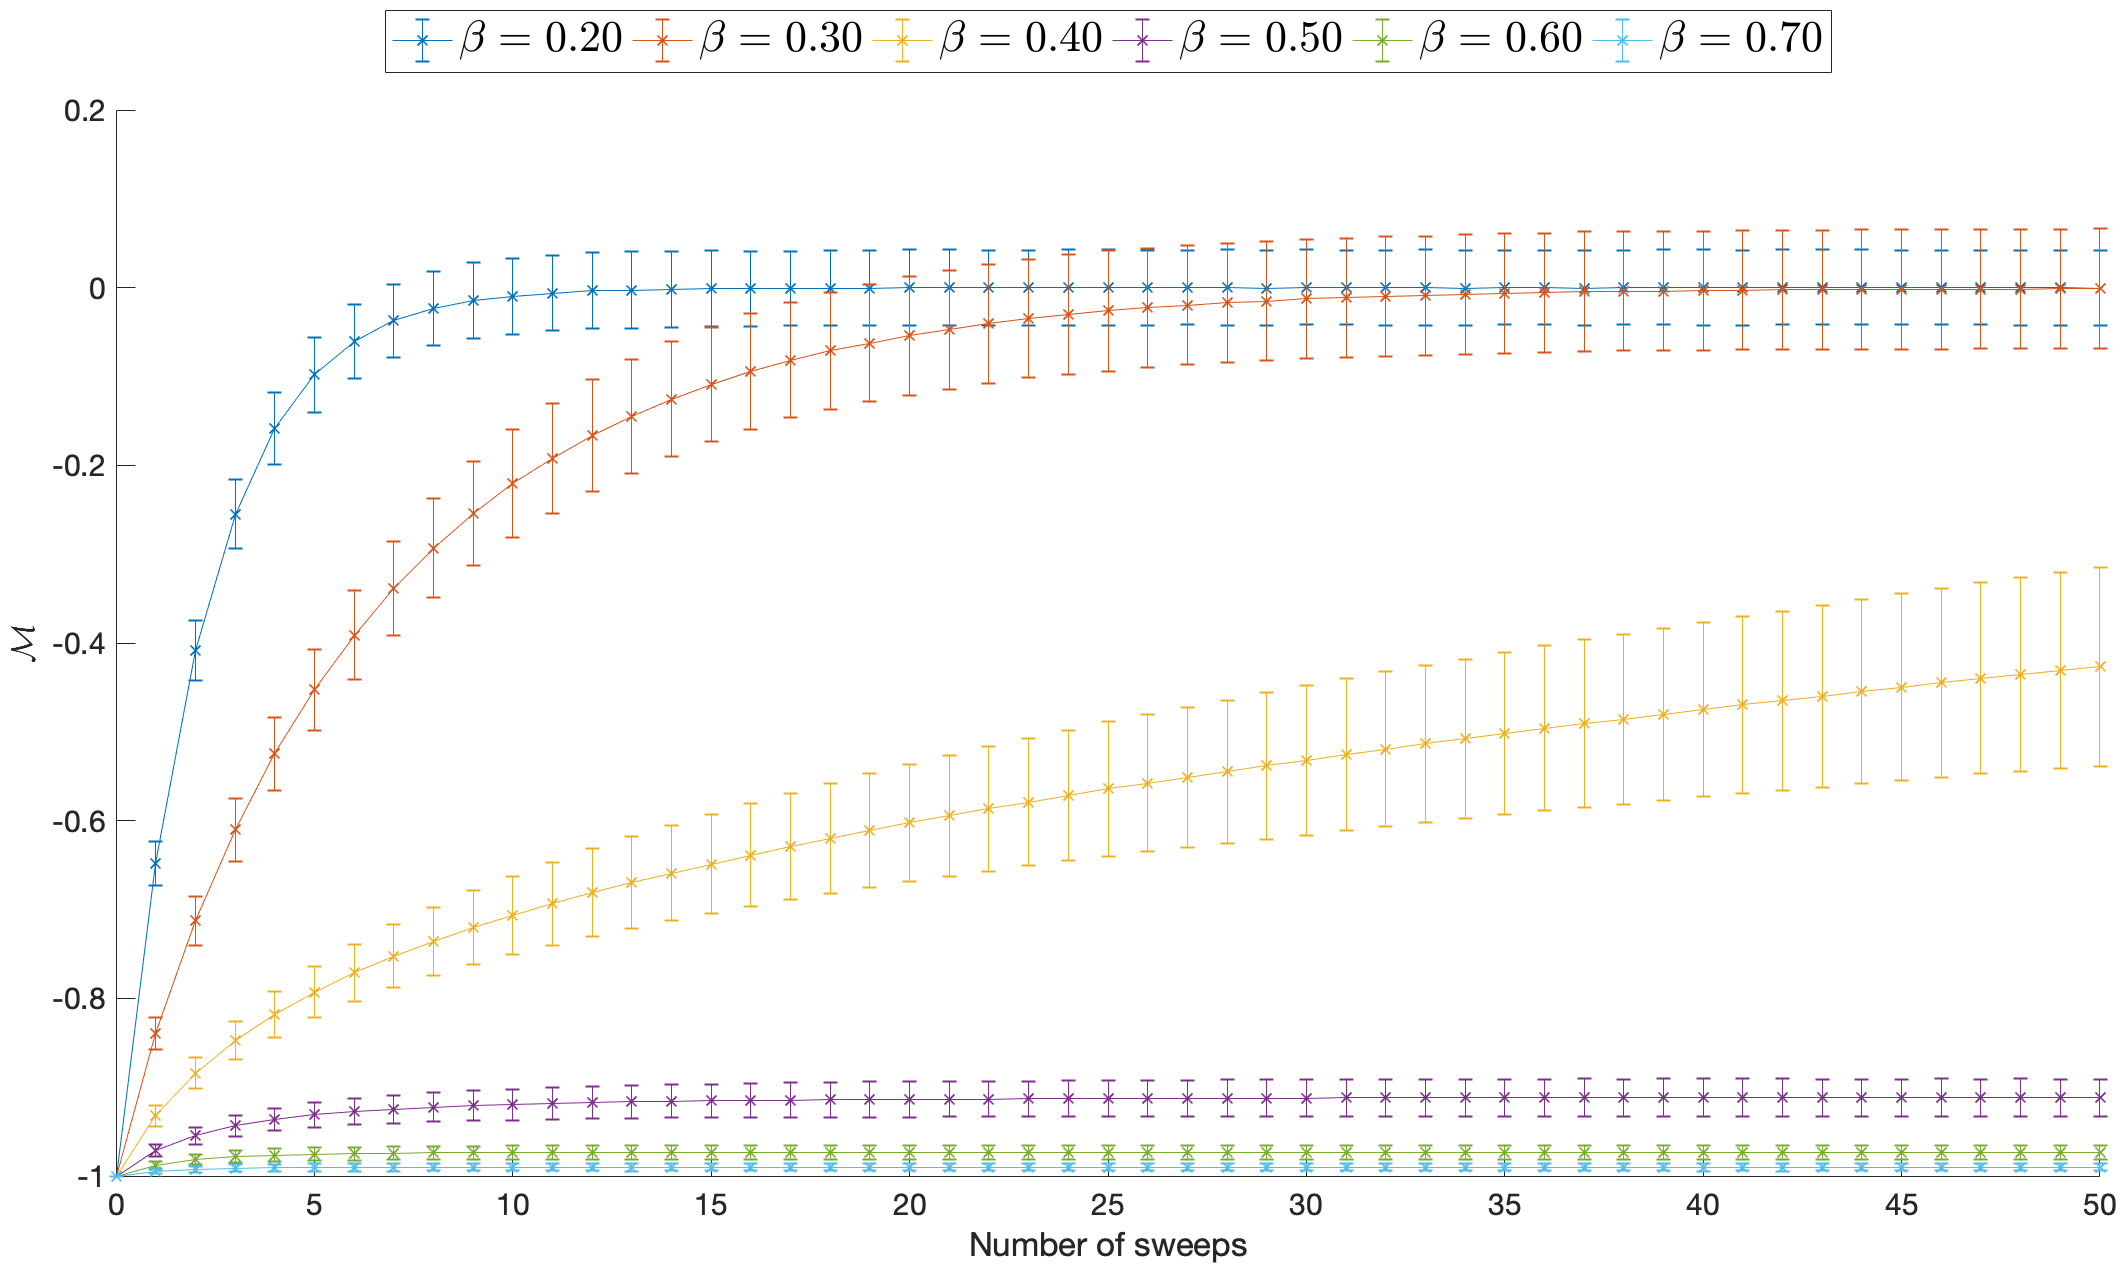
\includegraphics[width=0.8\linewidth]{images/section1/magnetisationfinal.png}
  \caption{Evolution of system magnetisation per spin as a function of the number of Monte Carlo sweeps completed for a 2D Ising model simulation with all spins initially down. The simulation was ran for a set of systems with different thermodynamic temperatures, as defined by the parameter $\beta$. Each data point represents the ensemble average over $n = 10,000$ independent sub-systems, each initialised with different pesudo-random number generator seeds. Error bars represent the standard deviation in the values of $\mathcal{M}$ across the ensemble of systems.}
  \label{fig:magnetisationconvergence}
\end{figure}

\begin{figure}[t]
  \centering
  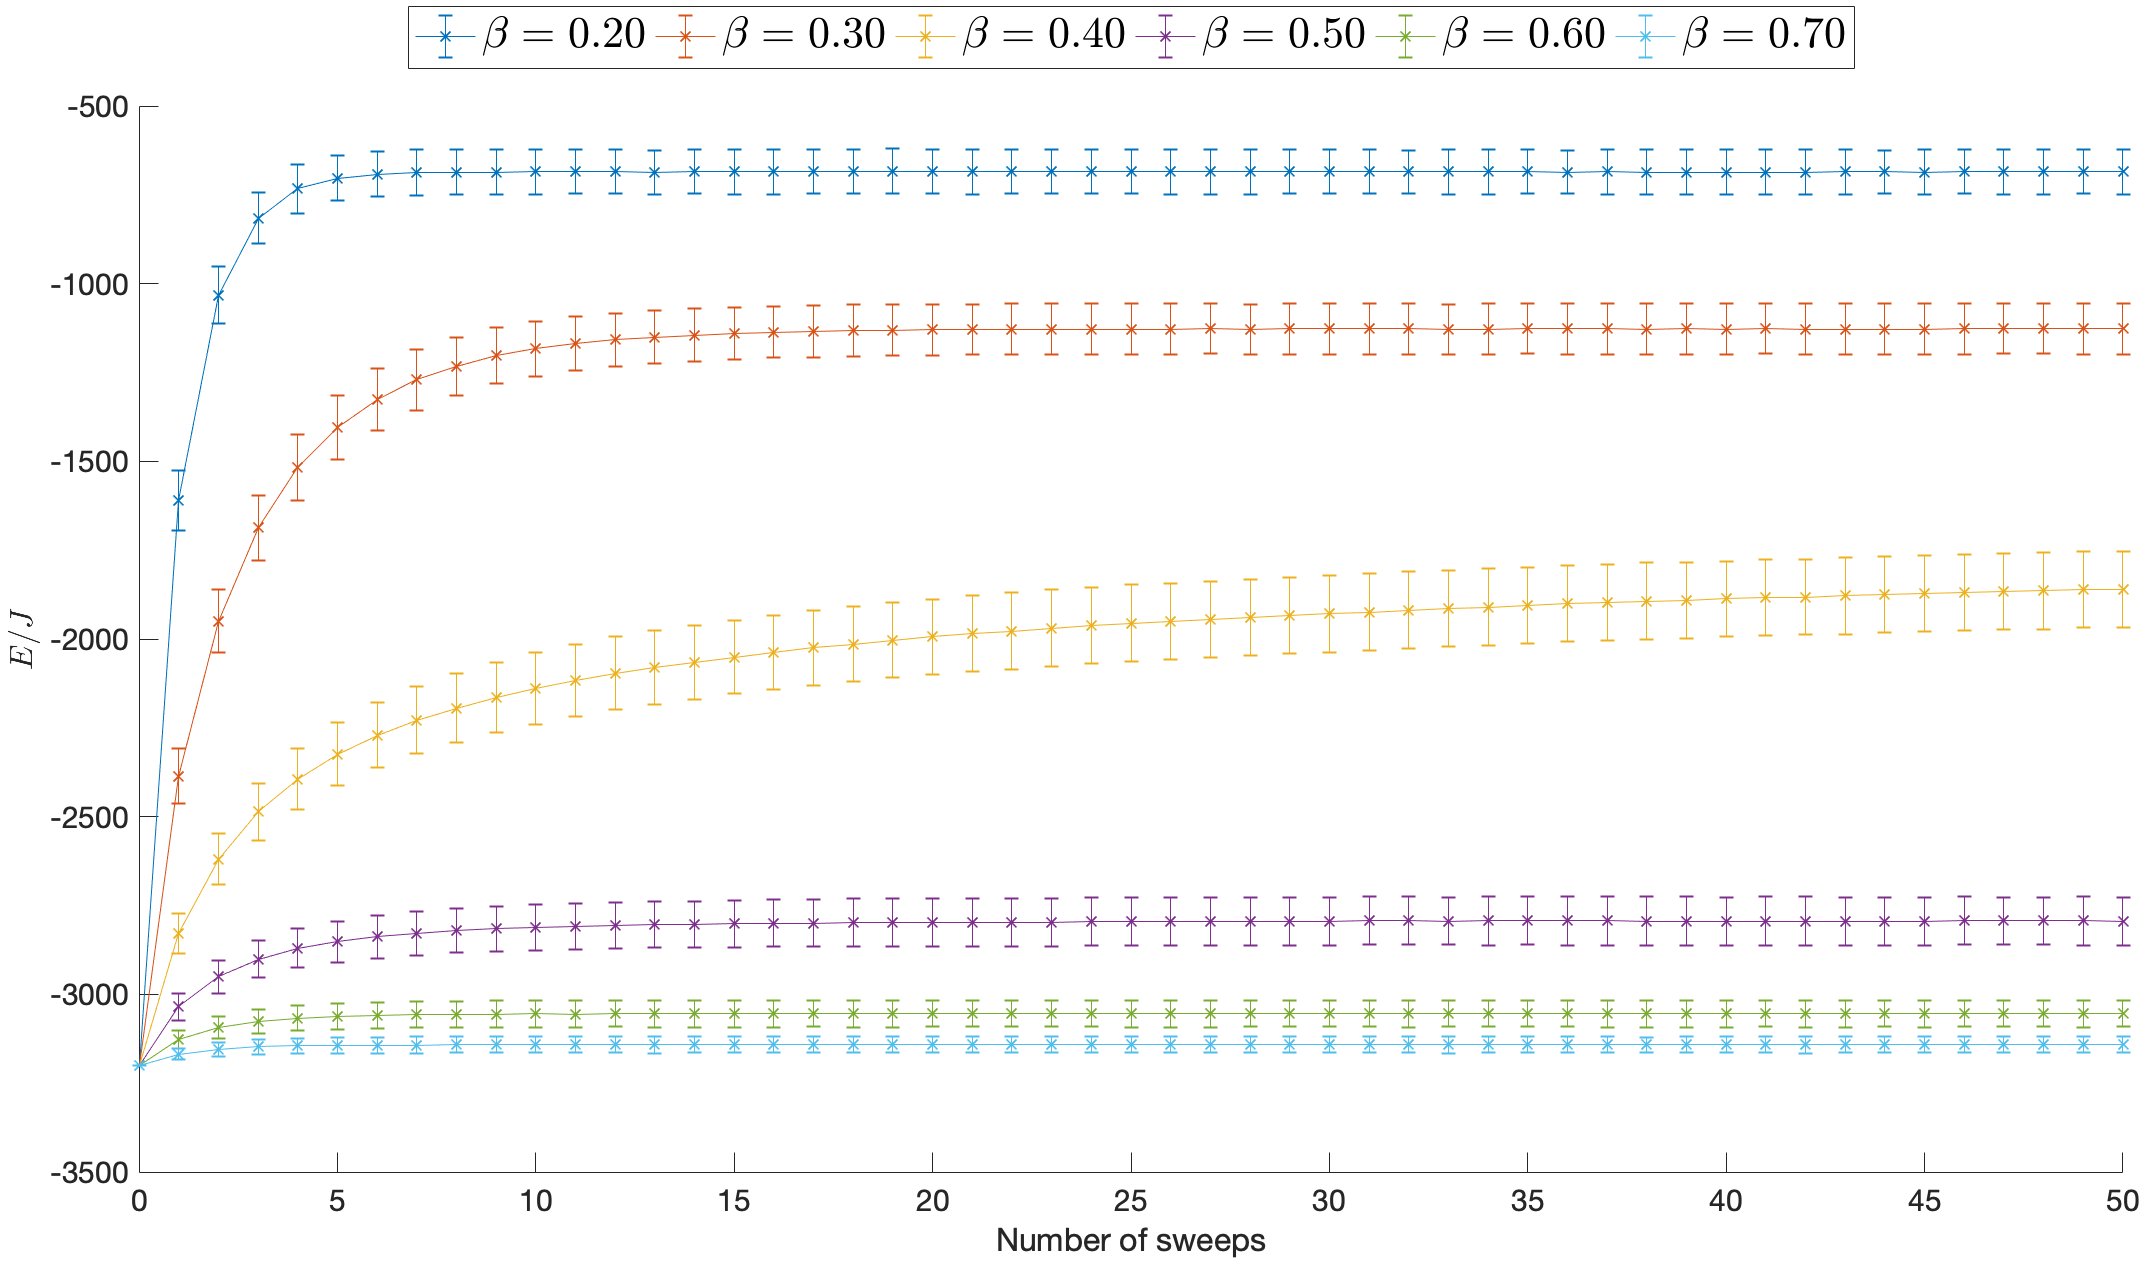
\includegraphics[width=0.8\linewidth]{images/section1/energyfinal.png}
  \caption{Evolution of dimensionless system energy as a function of the number of Monte Carlo sweeps completed for a 2D Ising model simulation with all spins initially down. The simulation was ran for a set of systems with different thermodynamic temperatures, as defined by the parameter $\beta$. Each data point represents the ensemble average over $n = 10,000$ independent sub-systems, each initialised with different pesudo-random number generator seeds. Error bars represent the standard deviation in the values for $E/J$ across the ensemble of systems.}
  \label{fig:energyconvergence}
\end{figure}

\subsection{Measuring Equilibrium Averages}

Figure \ref{fig:equilibriumaverages} shows averages of quantities of interest as a function of dimensionless temperature $T_0$ for an Ising system in thermal equilibrium. Figure \ref{fig:equilibriumaverages} (a) shows the average magnetisation per spin as a function of $T_0$. Figure \ref{fig:equilibriumaverages} (b) shows the average dimensionless energy per spin as a function of $T_0$. Figure \ref{fig:equilibriumaverages} (c) shows the average of the absolute value of the magnetisation per spin as a function of $T_0$. For each of these graphs, the average value of interest is sampled over $T_0 \in [1, 4]$ in discrete steps of $\Delta T_0 = 0.005$.

\begin{figure}[t]
    \centering
    \subfloat[Average magnetisation per spin]{{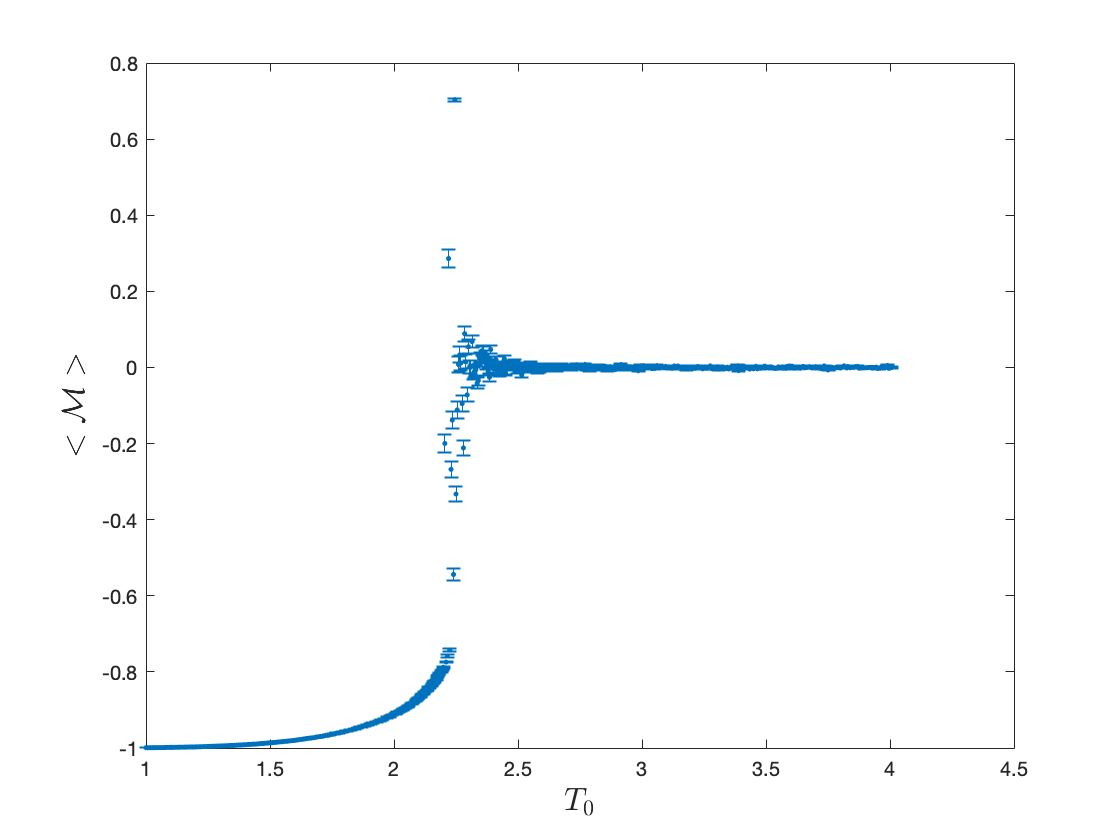
\includegraphics[width=8.11cm]{images/section2/magnetisationtime.png} }}\quad
     \subfloat[Average dimensionless energy per spin]{{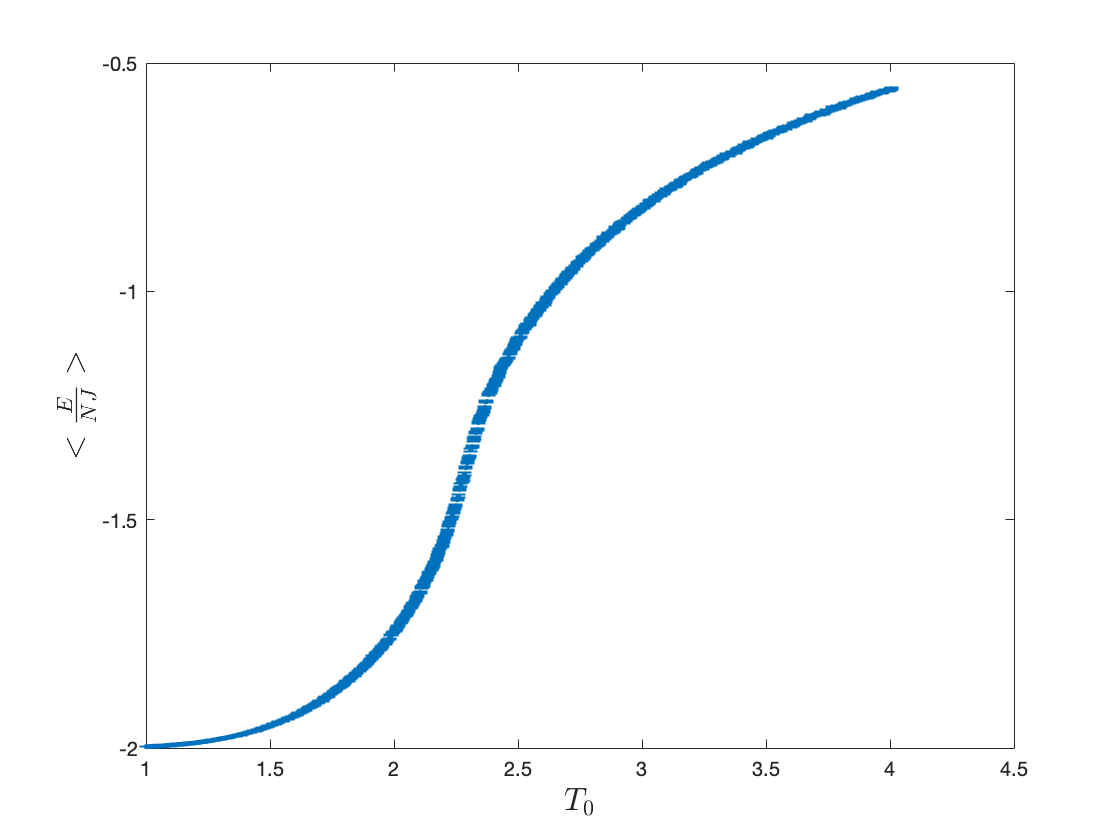
\includegraphics[width=8.11cm]{images/section2/energytime.png} }}\
          \subfloat[Average absolute magnetisation per spin]{{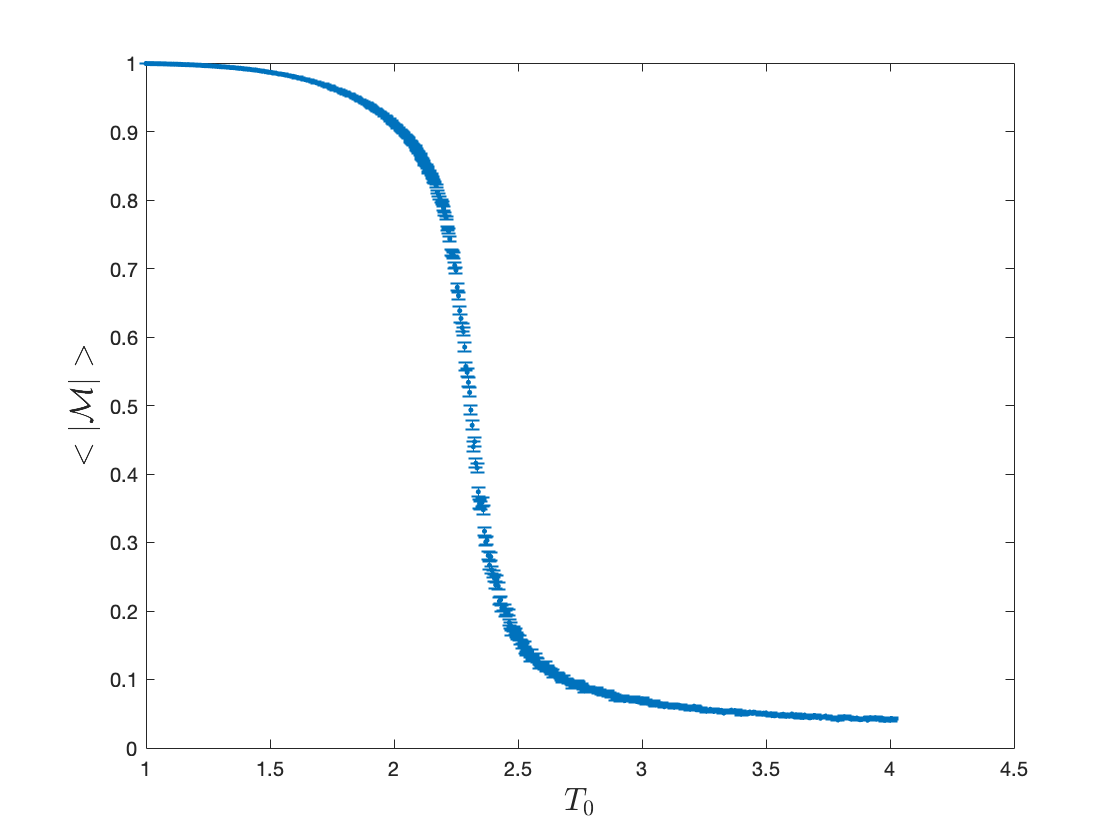
\includegraphics[width=8.11cm]{images/section2/absmagnetisation.png} }}\
 
    \caption{Averages of quantities as given by equation (\ref{eq:averages}) of interest as a function of dimensionless temperature $T_0$ for an Ising system in thermal equilibrium. (a) shows average magnetisation per spin $\langle\mathcal{M}\rangle$ vs $T_0$. (b) shows average dimensionless energy per spin $\langle\frac{E}{NJ}\rangle$ vs $T_0$. (c) shows average absolute magnetisation per spin $\langle|\mathcal{M}|\rangle$ vs $T_0$. Error bars represent standard errors as given by equation (\ref{eq:standarderror}).}
    \label{fig:equilibriumaverages}
\end{figure}

\subsection{Mean Field Theory}

Figure \ref{fig:meanFieldResults} shows the mean field theory results for quantities of interest in the Ising model. Figure \ref{fig:meanFieldResults} (a) shows mean field theory results for the magnetisation per spin. Figure \ref{fig:meanFieldResults} (b) shows results for the dimensionless energy per spin. Figure \ref{fig:meanFieldResults} (c) shows results for the dimensionless heat capacity. Figure \ref{fig:meanFieldResults} (d) shows results for the magnetic susceptibility.

\begin{figure}[t]
    \centering
    \subfloat[Magnetisation per spin]{{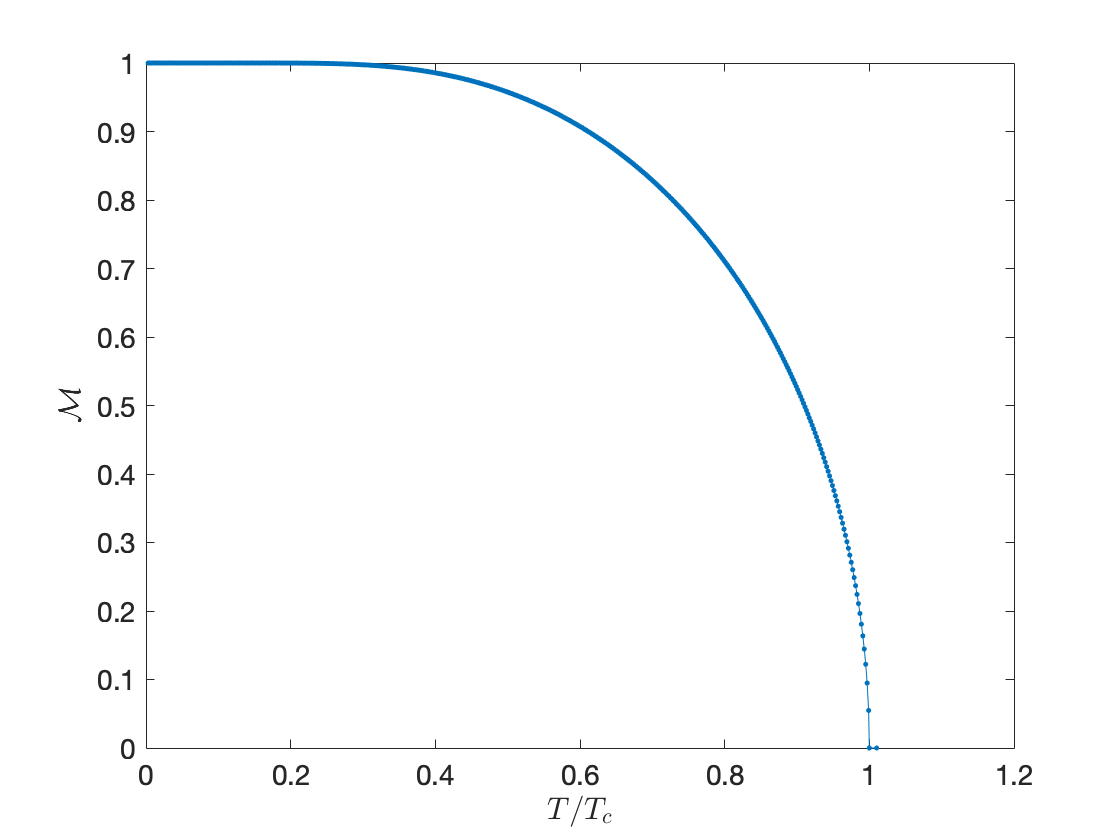
\includegraphics[width=8cm]{images/meanfield/magnetisation.png} }}\quad
     \subfloat[Dimensionless energy per spin]{{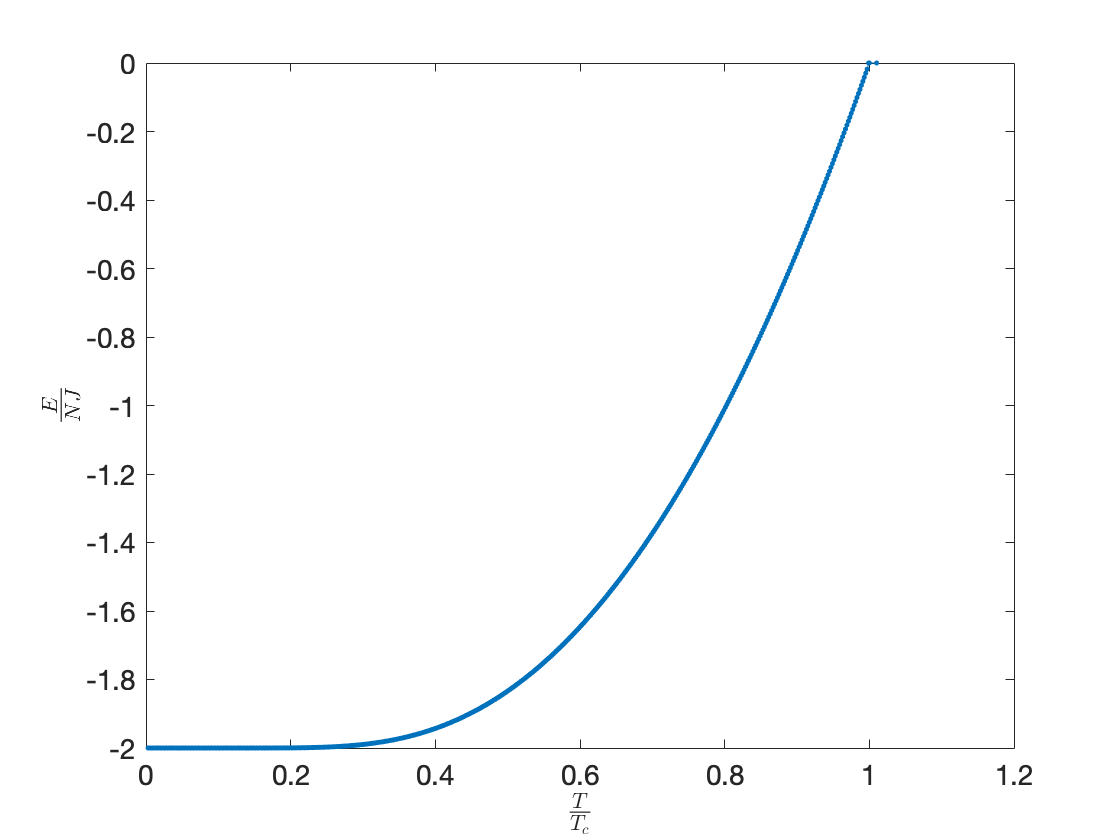
\includegraphics[width=8cm]{images/meanfield/energypersite.png} }}\\
     \subfloat[Dimensionless heat capacity]{{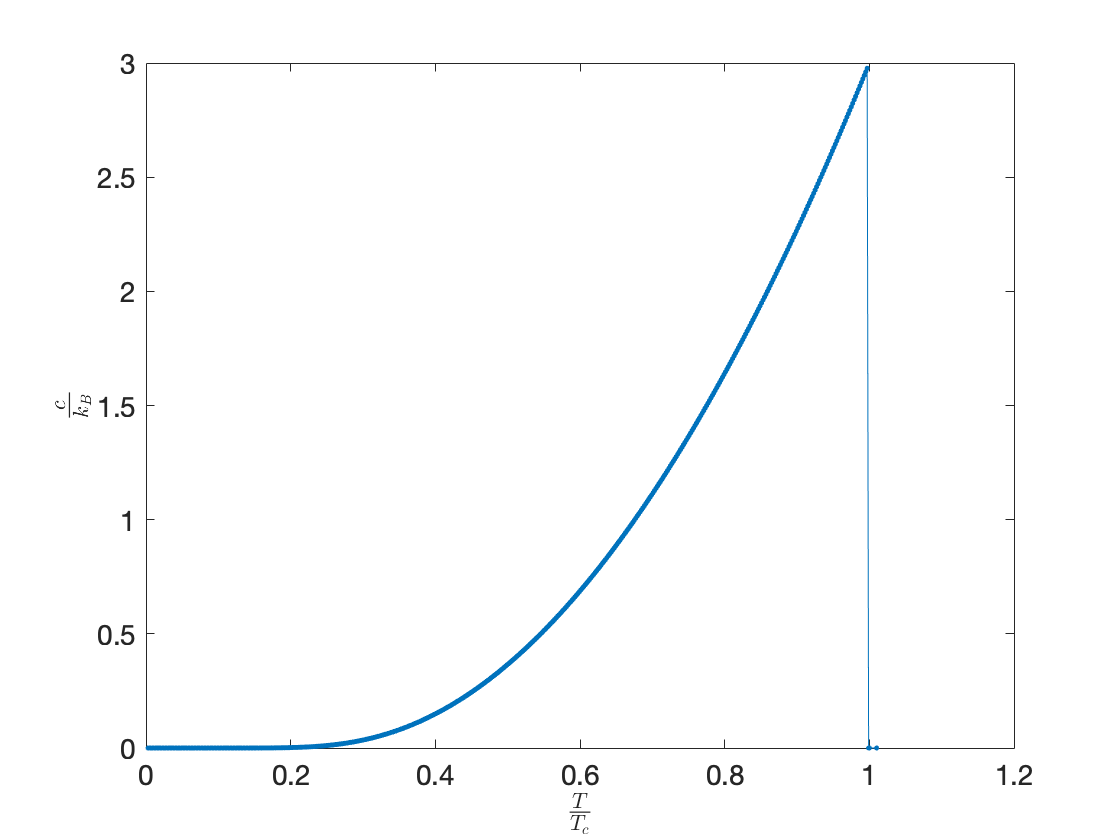
\includegraphics[width=8cm]{images/meanfield/heatcapacity.png} }}\quad
        \subfloat[Magnetic Susceptibility]{{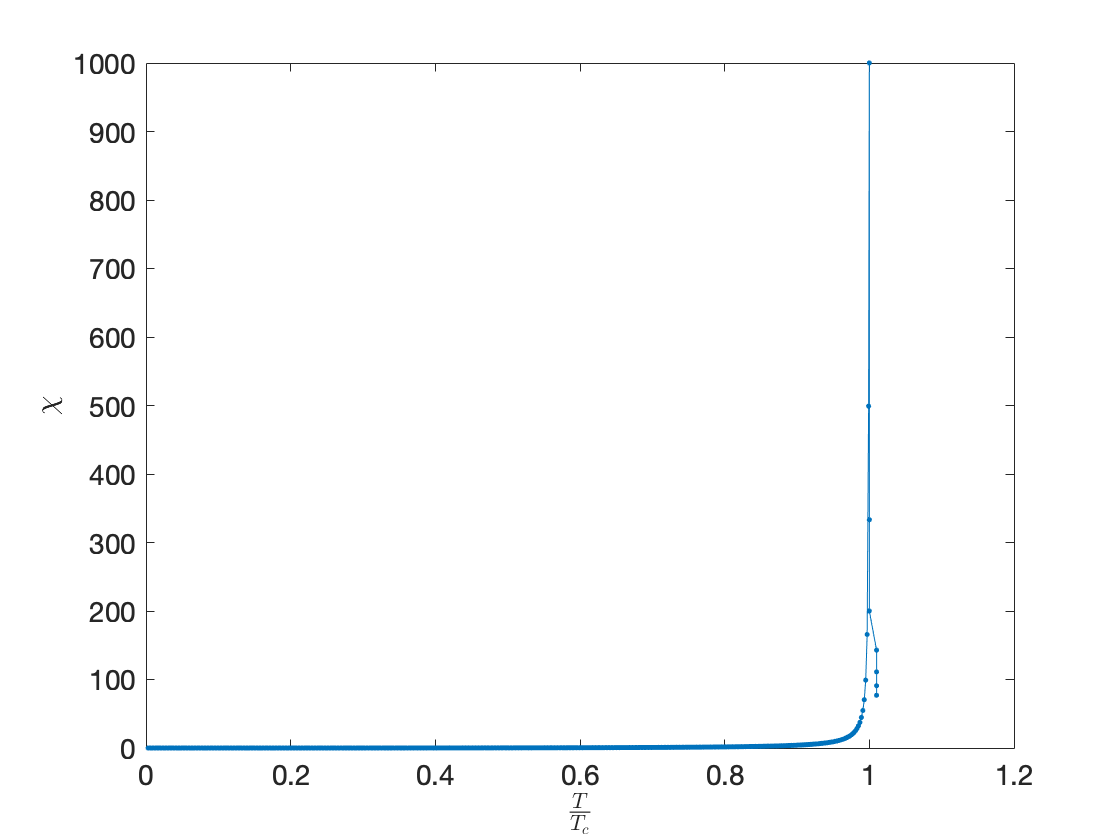
\includegraphics[width=8cm]{images/meanfield/chi.png} }}\quad
    \caption{TODO}
    \label{fig:meanFieldResults}
\end{figure}

\subsection{Specific Heat Capacitiy and Magnetic Susceptibility}

\begin{figure}[t]
    \centering
    \subfloat[]{{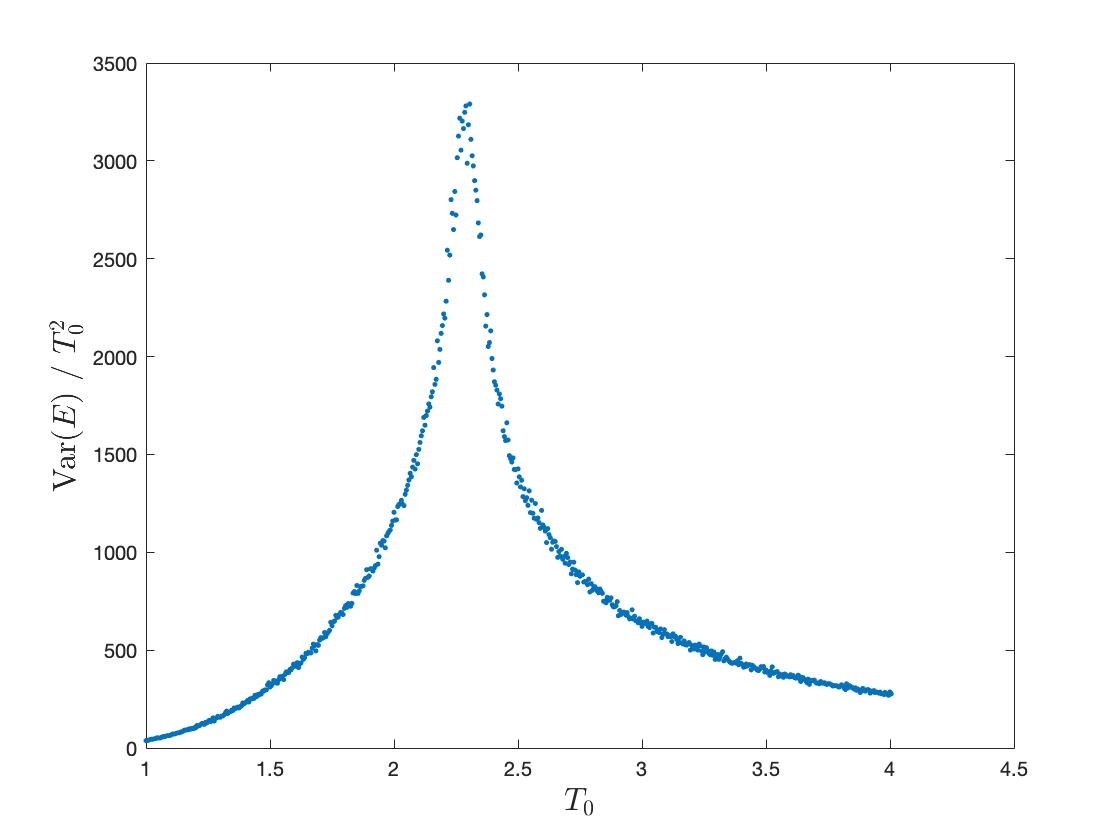
\includegraphics[width=8.11cm]{images/properties/varE.png} }}\quad
     \subfloat[]{{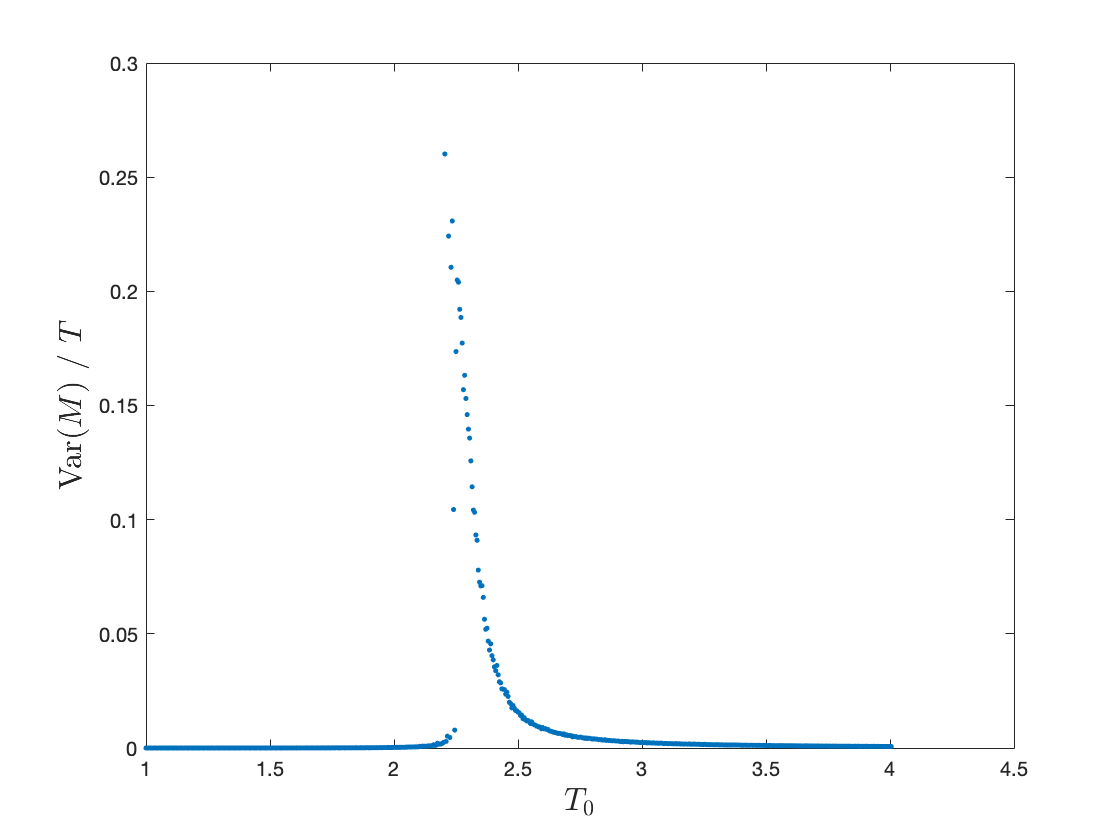
\includegraphics[width=8.11cm]{images/properties/varM.png} }}\
 
    \caption{}
    \label{fig:derivedproperties}
\end{figure}

\section{Discussion}
\subsection{Determining the Fractal Dimension of DLA Aggregates where $p_{stick} = 1$}
\subsection{Suggestions for Improvement}

\section{Conclusion}

\section*{References}
\bibliography{references}
\bibliographystyle{plain}

\end{document}

